\section{PreProject}
\subsection{Rich Picture}

\begin{figure}[h!]		%Remember to put the h!, to not fuck the sections.
 \begin{centering}
  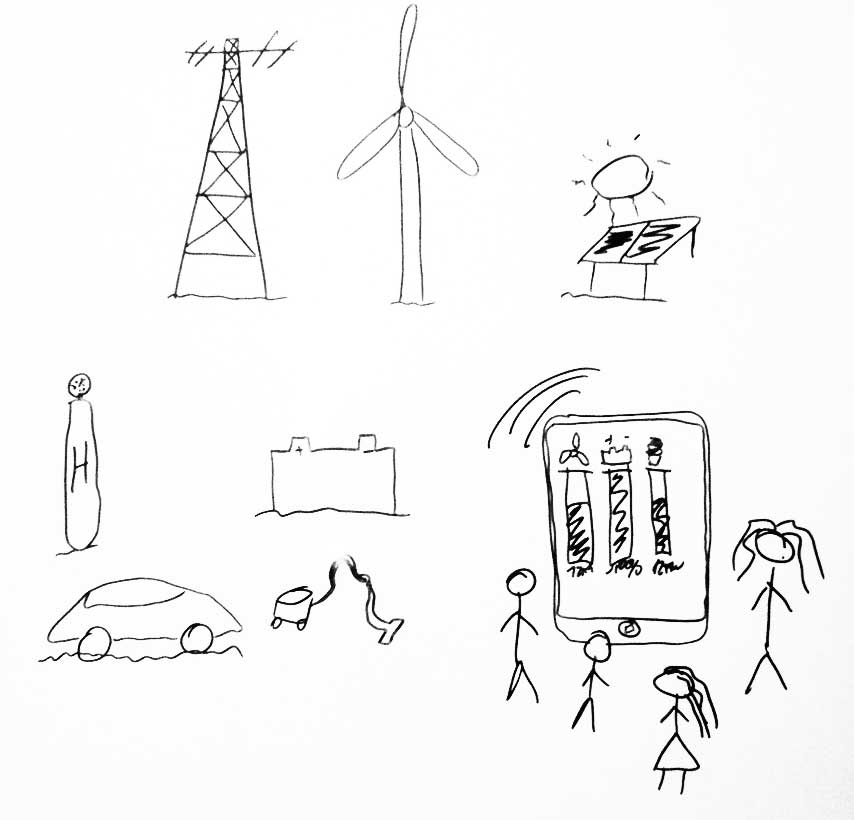
\includegraphics[width=1\textwidth]{images/rich_picture1.png}
   \caption{The surrounding environment is shown in the rich picture. The
 			 elements are: solar-panels, hydrogen storrage, battery-charger, windturbine
 			 converter, userinterface, the electric grid and different loads such as a
 			 hyrogen engine, vacumcleaner etc. }
 \end{centering}
\end{figure}

\subsection{Storry Telling}
Aarhus University, a place full of innovation and great ideas. Jan Nielsen
welcomes a class of high-school students to the green system simulator. Here it
is possible to see how much energy you can get out of green energy harvesting
such as wind and solar energy. When the system produces to much energy, the 
energy is stored in form of Hydrogen. The Hydrogen is to be used for a Hydrogen
driven engine which is placed nearby the green system simulator. Here people can
really come an get an idea about how much they can help the environment, but
also their own wallet, if they invest in some green energy for their own house.
The guests can navigate around on a screen to see how much energy each device 
creates or consumes, this is shown in a down to earth way, where everybody can follow, 
even persons without no special education or courses in the energy field.
\subsection{Storycards}
\textbf{Story Card 1:} I want to be able see how much energy is being harvest by
the wind turbines and solar panels and how much energy is being consumed, this should be
a user friandly graphycal interface.\\
\textbf{Story Card 2:} When the energy production is higher (batteries full
charged, and no loads connected), the energy should be stored as hydrogen in a safe way so
later it can be converted again to energy by a fuel cell or used as gas for a
hydrogen car.\\
\textbf{Story Card 3:} In order to show of, the interface has too be userfriedly
and easy too use, so students coming over to AU - Herning without any energy
knowledge should be able to easly navigate the system.\\
\textbf{Story Card 4:} The system will be in a outside enviroment, so it as to
be robust against weather conditions and people temper.\\
\textbf{Story Card 5:} When batteries and hydrogen tanks are fully charged, the
energy should be provided into the national power grid or/and university electrical
system.\\
\textbf{Story Card 6:} For further improvements and development the system have
to be fully documented, scalable and modular hardware construction.\\
\newpage
\subsection{Preliminary Use Cases}

\begin{figure}[!h]
	\begin{centering}
		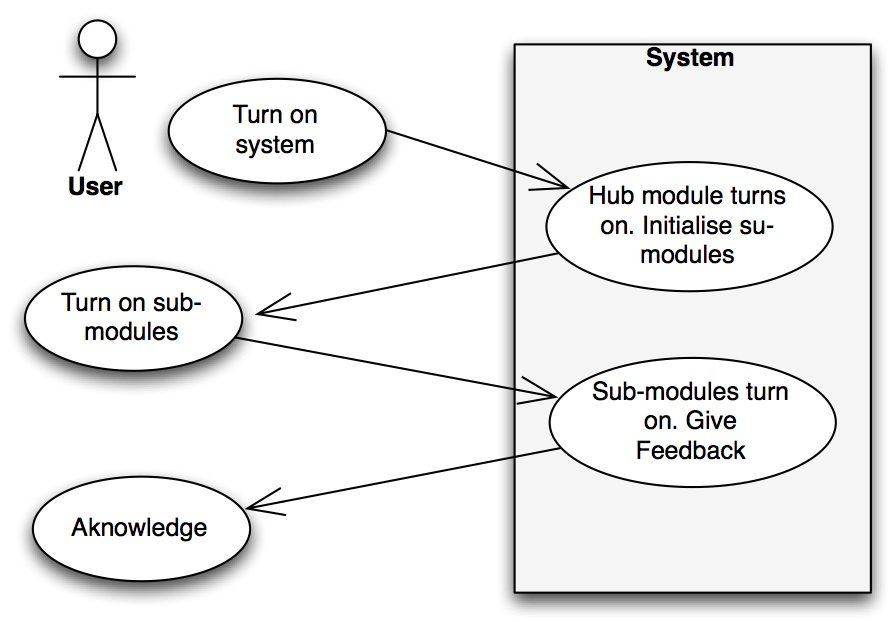
\includegraphics[width=0.7\textwidth]{images/usecases1.jpg}
		\caption{System initialisation. }
	\end{centering}
\end{figure}

\begin{figure}[!h]
	\begin{centering}
		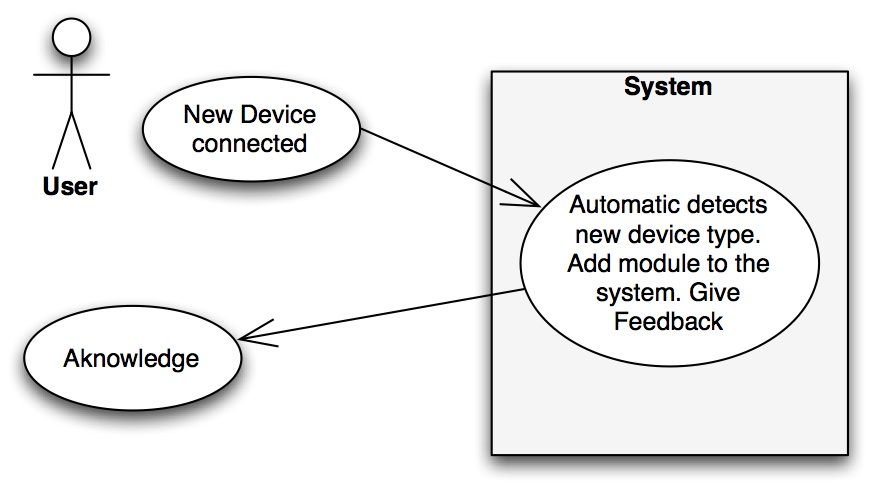
\includegraphics[width=0.7\textwidth]{images/usecases2.jpg}
		\caption{New device connected to the system. }
	\end{centering}
\end{figure}
\newpage

\subsection{Stakeholder Analysis}
Who is responsible for what ?\\[0.5cm]
\textbf{Project coordinators:}\\
Morten Opprud\\
Klaus Kolle\\
\\
\textbf{Customers/Users:}\\
Jan Nielsen - Customer ( Primary User )\\
High school students ( Secundary Users )\\
Rene A. S. Josefsen\\
\\
\textbf{Developers:}\\
Dennis Madsen\\
Theis Christensen\\
Pualo M. Fontes\\
\\
\textbf{Supliers:}\\
Jens Mortensen\\
Per Lysgaard\\
\\
\textbf{Theory Advicers:}\\
Henning Slavensky\\
Ulrich Bjerre\\
Kristian Lomholdt\\

\begin{figure}[h!]
 \begin{centering}
  \begin{tabular}{| l | l | l |}
   \hline
      & Has decision power & Has no decision power \\ \hline
    Directly involved stakeholder & Jan Nielsen, Developers & Klaus Kolle,
    Morten Opprud \\ \hline Not directly involved stakeholder & High School Students & Jens
    Mortensen, Per Lysgaard \\
    \hline
   \end{tabular}
  \end{centering}
 \caption{Stakeholder table}
\end{figure}

\textbf{Why this selection:}
Klaus Kolle and Morten Opprud, are the project coordenators so they have no
decision power over the customers choice.
\\
Jan Nielsen is the customer, the primary user so he has decision power over the
final product.
\\
High School Students have decision power over the final interface since, they
are the secondary users of the system.

\subsection{System Definition}
\textbf{Proposal 1 - Fully automatically}\\
The Energy-Hub system is the central device in the green-energy system. All
inputs and output devices is automatically routed to the right place inside this
device. That means when devices is connected to the Energy HUB, it automatically
sees if it is an input or an output unit. On the web-page of the module the user
have the possibility of using between two modes:
\\ - Green System profile.
\\ - Fast charging profile.
\\The Green profile only makes use of the green power devices such as
voltaic-cells, wind power, energy from the charged batteries or from the
hydrogen tank. 
The fast charging profile on the other hand charges the hydrogen tank and the
battery on the fastest possible way. In other words, if there is not enough
green energy, energy will be taken from the grid.
\\If we are in a condition where the hydrogen and battery storages are full,
then energy produced becide this will be sent to the grid or go to the schools
electrical system.
\\\textbf{Proposal 2:}\\
To switch between the green mode to fast charging a button can be putted
physicaly in the hardware box.\\
\\\textbf{Proposal 3 (Optimizing):}\\
Extra output extension model that the user can connect devices, and switch
each output on and off. This can be used to present to high school students
the navigation trought the system using some physical actions.